\documentclass[twocolumn]{article}

%\usepackage[italian]{babel}
\usepackage{graphicx}
\usepackage{amsmath,amsfonts,amssymb}
\usepackage{hyperref}   % per \url

% per fare i diagrammi
\usepackage{tikz}
\usetikzlibrary{angles, quotes, calc}


% rimuove l'indentazione all'inizio dei paragrafi e aggiunge spazio tra i paragrafi
\setlength{\parindent}{0pt}
\setlength{\parskip}{6pt}   % risistemare alla fine!!!!

\title{Relazione 1}

\author{
Luca Vettore, Enrico Vianelli, Lorenzo Zanoli
}

\date{\today}

\begin{document}

\maketitle

\section{Introduzione}
Lo scopo di questa analisi è quello di determinare attraverso tecniche di inferenza bayesiana alcuni dei parametri che descrivono la cinematica della Via Lattea. In particolare abbiamo stimato la velocità tangenziale di rotazione delle stelle attorno al centro galattico (CG), $V_{rot}$, e le componenti della velocità del sole rispetto al Local Standard of Rest (LSR), $U_\odot$, $V_\odot$ e $W_\odot$.


\subsection{I dati: GAIA DR2}

Questo lavoro si basa su dati forniti dalla missione {\it Gaia} (\url{https://www.cosmos.esa.int/gaia}) del European Space Agency (ESA), processati dal {\it Gaia} Data Processing and Analysis Consortium (DPAC, \url{https://www.cosmos.esa.int/web/gaia/dpac/consortium}). I fondi per il DPAC sono stati forniti da istituzioni nazionali, in particolare le istituzioni partecipanti al {\it Gaia} Multilateral Agreement.

% controllare siano davvero 3 milioni!!!
In particolare, abbiamo utilizzato i dati della terza release (DR3) di {\it Gaia}, che include informazioni su $3000000$ di stelle della via lattea. La nostra analisi utilizza la latitudine $l$ e longitudine $b$ galattica, la parallasse $\varpi$ e la velocità lungo la linea di vista $V_{rad}$, con i relativi errori.


\subsection{Le coordinate galattiche e i parametri cinematici}
L'analisi utilizza il sistema di coordinate galattiche, cioè un sistema di coordinate sferiche centrato sul sole in cui la longitudine $l$ è misurata a partire dal centro galattico (CG) e la latitudine $b$ misura l'angolo di elevazione rispetto al piano galattico.

La parallasse $\varpi$ rappresenta lo spostamento apparente di una stella quando osservata da punti opposti dell'obita terrestre e permette di stimare la distanza $d$ della stella attraverso la relazione $d = 1/\varpi$ (con $\varpi$ espressa in arcosecondi e $d$ in parsec).

La velocità del sole rispetto al LSR è rappresentata dalle componenti ($U_\odot$, $V_\odot$, $W_\odot$), dove $U_\odot$ è la componente radiale (verso il CG), $V_\odot$ è la componente tangenziale (nella direzione di rotazione) e $W_\odot$ è la componente verticale (verso il polo nord galattico). La velocità di rotazione $V_{rot}$ rappresenta la velocità tangenziale media delle stelle attorno al CG.


\subsection{Il modello}

% capire se mettiamo la versione 2D, 3D o entrambe

I dati {\it Gaia} includono la velocità radiale $V_{rad}$, che è la componente della velocità di una stella lungo la linea di vista. Questa velocità può essere modellata come la somma di due componenti: una dovuta al moto peculiare del sole rispetto al LSR, $V_{rad}^{LSR}$, e una dovuta alla rotazione della galassia, $V_{rad}^{ROT}$.

Limitandoci al piano galattico ($b=0$), il contributo della rotazione galattica può essere calcolato passando per la differenza di velocità angolare tra la stella in esame e il sole:

\[ \Delta\omega = \left(\frac{V_{rot}}{R_\odot} - \frac{V_{rot}}{R_i}\right) \Rightarrow V_{rot}^{rel} = \Delta\omega \cdot R_i \].

Dove $R_\odot\simeq 8.12$ kpc è la distanza del sole dal CG e $R_i$ è la distanza della stella i-esima dal CG.

I valori di $R_i$ e $V_{ROT}$ possono essere ricavati dalla geometria del sistema, come mostrato in Figura \ref{fig:measures}, ottenendo le relazioni:

% controllare le formule anche se dovrebbero andare bene
\[ R_i = \sqrt{d^2+R_\odot^2 - 2dR_\odot\cos(l)} \]
\[ V_{ROT} = V_{rot} \left( \frac{R_\odot}{R_i} - 1 \right) \sin(l). \]

% Diagramma della costruzione geometrica per le proiezioni e il calcolo degli angoli.
% un triangolo con il sole, il cg e una stella. I lati del triangolo solo R_\odot, R_i e d. Gli angoli sono l tra R_\odot e d, \alpha tra R_i e d, e \beta il complementare di \alpha
% V_rad è diretta lungo d, V_rot^rel lungo la perpendicolare ad R_i.
\begin{figure}

    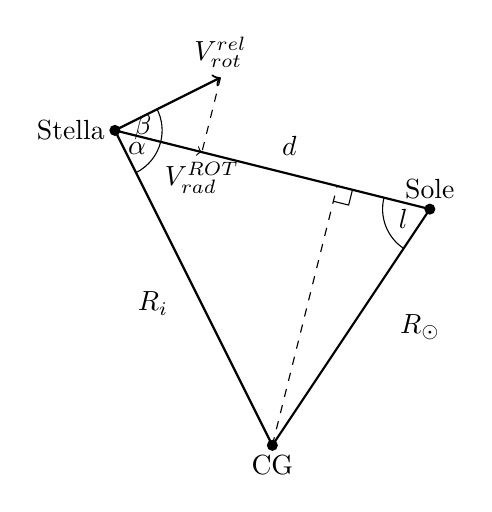
\begin{tikzpicture}
        % dbg grid
        %\draw[help lines] (-1,-1) grid (5,5);
    
        % nodi con nomi
        \coordinate (CG)   at (2,0);
        \coordinate (Sole) at (4,3);
        \coordinate (Stella) at (0,4);
    
        % triangolo
        \draw[thick] (CG) node[below] {CG}
                  -- (Sole) node[above] {Sole}
                  -- (Stella) node[left] {Stella}
                  -- cycle;
        
        % punti ai vertici
        \fill (CG) circle (2pt);
        \fill (Sole) circle (2pt);
        \fill (Stella) circle (2pt);
    
        % nomi lati
        \node at (3.5,1.5) [right] {$R_\odot$};
        \node at (0.8,1.8) [left]  {$R_i$};
        \node at (2,3.8)   [right] {$d$};
    
        % vettori velocità
        \coordinate (Vt) at ($(Stella)!1.5cm!90:(CG)$);
        \draw[->, thick] (Stella) -- (Vt) node[above] {$V_{rot}^{rel}$};
    
        % proiezione di Vt su d
        \coordinate (Vt_proj) at ($(Stella)!(Vt)!(Sole)$);
        \draw[-, dashed] (Vt) -- (Vt_proj) node[above] {};
        \draw[->, dashed] (Stella) -- (Vt_proj) node[below] {$V^{ROT}_{rad}$};
    
        % altezza del triangolo (da CG)
        \coordinate (H) at ($(Stella)!(CG)!(Sole)$);
        \draw[-, dashed] (CG) -- (H) node[above] {};
    
    
        % angoli
        \draw pic["$l$",     draw, angle radius=0.6cm] {angle = Stella--Sole--CG};
        \draw pic["$\alpha$",draw, angle radius=0.6cm] {angle = CG--Stella--Sole};
        \draw pic["$\beta$", draw, angle radius=0.6cm] {angle = Sole--Stella--Vt};
        \draw pic[draw, angle radius=0.2cm] {right angle = Sole--H--CG};
        
        
    \end{tikzpicture}
    \caption{Costruzione geometrica per il calcolo delle velocità nel piano galattico.}\label{fig:measures}
    
\end{figure}

Il contributo dovuto al moto peculiare del sole rispetto al LSR, $V_{rad}^{LSR}$, può essere calcolato proiettando le componenti della velocità del sole lungo la linea di vista:
\[ V_{rad}^{LSR} = U_\odot \cos(l) + V_\odot \sin(l). \]

L'estensione del modello al caso tridimensionale, con $b \neq 0$, è immediata e porta a modificare le formule di $V_{rad}^{LSR}$ e $V_{rad}^{ROT}$ introducendo i fattori $\cos(b)$ e $\sin(b)$ per tenere conto della latitudine galattica. In particolare, si ottiene:

% controllare le formule!!!!!
\begin{align*}
    &V_{rad}^{LSR} = U_\odot \cos(l) \cos(b) + V_\odot \sin(l) \cos(b) + W_\odot \sin(b)\\
    &V_{rad}^{ROT} = V_{rot} \left( \frac{R_\odot}{R_i} - 1 \right) \sin(l) \cos(b)\\
    &V_{rad} = V_{rad}^{LSR} + V_{rad}^{ROT}.
\end{align*}


% controllare anche i nomi delle sezioni. Un'opzione forse migliore sarebbe fare una sezione modello divisa in modello fisico e modello statistico.
\section{Analisi statistica: MCMC e inferenza bayesiana}
Per stimare i parametri del modello, è stata adottata una procedura di inferenza bayesiana basata su Markov Chain Monte Carlo (MCMC), implementata attraverso la libreria \texttt{emcee}. L'obiettivo è quello di campionare la distribuzione a posteriori dei parametri $V_{rot}$, $U_\odot$, $V_\odot$ e $W_\odot$ dato il dataset di {\it Gaia}.

La funzione di verosimiglianza è stata definita assumendo errori gaussiani indipendenti sui dati di $V_{rad}$ forniti da {\it Gaia}. La deviazione standard totale $\sigma_{tot}$ è stata calcolata combinando l'errore riportato da {\it Gaia} con l'incertezza derivante dalla misura della parallasse, attraverso la formula:
\[ \sigma_{tot} = \sqrt{\sigma_{Gaia}^2 + \left( \frac{\partial V_{rad}}{\partial \varpi} \sigma_\varpi \right)^2}. \]
% vogliamo aggiungere anche la sigma intrinsenca che avevamo messo all'inizio? A questo punto sarebbe solo un termine additivo e un parametro in più nell'inferenza

Il valore di $\frac{\partial V_{rad}}{\partial \varpi}$ dipende da $V_{rot}$. Per questo motivo abbiamo diviso l'analisi in due fasi:
\begin{itemize}
    \item Nella prima fase abbiamo inizializzato i walker con valori casuali (propagando l'errore usando un valore fissato di $V^*_{rot} = 100 km/s$). Lo scopo di questa fase è quello di identificare la zona ad alta probabilità della distribizione a posteriori e permettere una stima più accurata di $V^*_{rot}$ da usare nella seconda fase.
\end{itemize}





\end{document}